\subsection{Extending the Interface}
\label{sec:extending-interface}
With the \code{ArrowParallel} typeclass in place and implemented, we can now implement some further basic parallel interface functions. These are algorithmic skeletons that, however, mostly serve as a foundation to further, more specific algorithmic skeletons.

\subsubsection{Lazy \code{parEvalN}}
\begin{figure}[h]
	\includegraphics[scale=0.7]{images/parEvalNLazy}
	\caption{Schematic depiction of parEvalNLazy}
	\label{fig:parEvalNLazyImg}
\end{figure}
The function \code{parEvalN} is 100\% strict, which means that it fully evaluates all passed arrows. Sometimes this might not be feasible, as it will not work on infinite lists of functions like e.g. \code{map (arr . (+)) [1..]} or just because we need the arrows evaluated in chunks. \code{parEvalNLazy} (Fig.~\ref{fig:parEvalNLazyImg},~\ref{fig:parEvalNLazy}) fixes this. It works by first chunking the input from \code{[a]} to \code{[[a]]} with the given \code{ChunkSize} in \code{arr (chunksOf chunkSize)}. These chunks are then fed into a list \code{[arr [a] [b]]} of parallel arrows created by feeding chunks of the passed \code{ChunkSize} into the regular parEvalN by using \code{listApp} (Fig.~\ref{fig:listApp}). The resulting \code{[[b]]} is lastly converted into \code{[b]} with \code{arr concat}.
\begin{figure}[h]
\begin{lstlisting}[frame=htrbl]
parEvalNLazy :: (ArrowParallel arr a b conf, ArrowChoice arr, ArrowApply arr) =>
	conf -> ChunkSize -> [arr a b] -> (arr [a] [b])
parEvalNLazy conf chunkSize fs =
	arr (chunksOf chunkSize) >>>
	listApp fchunks >>>
	arr concat
	where fchunks = map (parEvalN conf) $ chunksOf chunkSize fs
\end{lstlisting} %$ %% formatting
\caption{Definition of parEvalNLazy}
\label{fig:parEvalNLazy}
\end{figure}

\subsubsection{Heterogenous tasks}
\begin{figure}[h]
	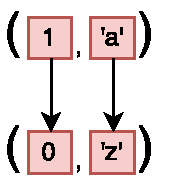
\includegraphics[scale=0.7]{images/parEval2}
	\caption{Schematic depiction of parEval2}
	\label{fig:parEval2Img}
\end{figure}
We have only talked about the paralellization arrows of the same type until now. But sometimes we want to paralellize heterogenous types as well. However, we can implement such a \code{parEval2} combinator (Fig.~\ref{fig:parEval2Img},~\ref{fig:parEval2}) which combines two arrows \code{arr a b} and \code{arr c d} into a new parallel arrow \code{arr (a, c) (b, d)} quite easily with the help of the \code{ArrowChoice} typeclass. The idea is to use the \code{+++} combinator which combines two arrows \code{arr a b} and \code{arr c d} and transforms them into \code{arr (Either a c) (Either b d)} to get a common arrow type that we can then feed into parEvalN.
\\\\
We start by transforming the \code{(a, c)} input into a 2-element list \code{[Either a c]} by first tagging the two inputs with \code{Left} and \code{Right} and wrapping the right element in a singleton list with \code{return} so that we can combine them with \code{arr (uncurry (:))}. Next, we feed this list into a parallel arrow running on 2 instances of \code{f +++ g} as described above. After the calculation is finished, we convert the resulting \code{[Either b d]} into \code{([b], [d])} with \code{arr partitionEithers}. The two lists in this tuple contain only 1 element each by construction, so we can finally just convert the tuple to \code{(b, d)} in the last step.
\begin{figure}[h]
\begin{lstlisting}[frame=htrbl]
parEval2 :: (ArrowChoice arr,
	ArrowParallel arr (Either a c) (Either b d) conf) =>
	conf -> arr a b -> arr c d -> arr (a, c) (b, d)
parEval2 conf f g = 
	arr Left *** (arr Right >>> arr return) >>>
	arr (uncurry (:)) >>>
	parEvalN conf (replicate 2 (f +++ g)) >>>
	arr partitionEithers >>>
	arr head *** arr head
\end{lstlisting}
	\caption{Definition of parEval2}
	\label{fig:parEval2}
\end{figure}


%%% Local Variables:
%%% mode: latex
%%% TeX-master: "main"
%%% End:
